\subsection{Emulation par limitation}
\label{section:limitation}
%% \begin{itemize}
%% \item principe: limiter l'accès aux ressources par exemple (cgroup, netstat, cpuburner), temps d'un SEB (bench avec netlink, limiter (cap))
%% \item avantage plus simple
%% \item désavantages: host>>target, modèle à vérifier, contrôle expérimental fin
%% \end{itemize}

Avec cette première méthode, illustrée Figure \ref{Virtu_limitation}, on place
la couche d'émulation au-dessus de la plateforme réelle (comme un hyperviseur
pour une VM). De fait, la puissance de l'émulateur dépend de la puissance de la
machine hôte et ne peux donc pas dépasser les capacités de cette dernière. De
plus, en choisissant de placer l'émulation comme une surcouche, cela permet de
limiter l'accès aux ressources pour les applications. En effet, elles ne
pourront pas passer la couche d'émulation pour accéder aux ressources localisées
sur la machine hôte. Les requêtes des applications seront arrêtées par
l'émulateur. C'est lui qui s'occupera de récupérer les ressources demandées par
les applications. Il existe différents outils permettant de mettre en place
cette virtualisation, on trouve notamment \textbf{cgroups} \citep{cgroups} et
\textbf{cpuburner} \citep{canon2006wrekavoc, buchert2011methods} pour le système
et \textbf{iptables} \citep{netfilter_iptables, iptables_man} pour le
réseau. L'émulation par limitation a l'avantage d'être simple à mettre en \oe
uvre puisque l'on se base sur la machine hôte. Néanmoins, elle est assez
contraignante du fait qu'on ne puisse pas émuler des architectures plus
performantes que l'hôte.

\begin{figure}[H]
  \centering
  \begin{subfigure}{0.3\textwidth}
    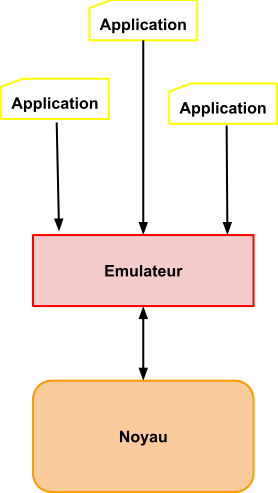
\includegraphics[scale=0.38]{Pictures/png/Virtualisation_limitation}
    \caption{Virtualisation par limitation.}
    \label{Virtu_limitation}
  \end{subfigure}
  \begin{subfigure}{0.4\textwidth}
    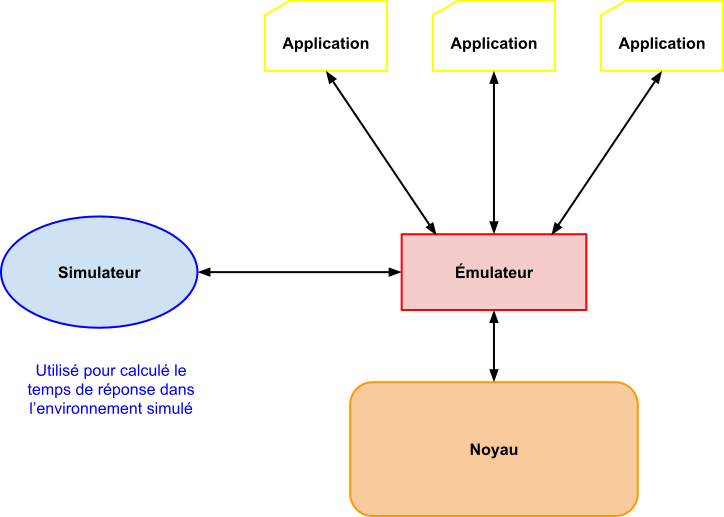
\includegraphics[scale=0.3]{Pictures/png/Virtualisation_interception}
    \caption{Virtualisation par interception.}
    \label{Virtu_interception}
  \end{subfigure}
  \caption{Approches de virtualisation légère.}
  \label{TYPE_VIRTUALISATION}
\end{figure}
